\section{Introduction}\label{sec:introduction}
SQLite clients updating independent databases and NATS JetStream connections publishing to different streams must wait for durable completion before processing subsequent requests.
Although these updates have no data dependencies across files, the filesystem can make them compete for the same append position.
As concurrency increases, shared allocation state becomes a serialization point on the application's persistence path.

Zoned Namespace (ZNS) solid-state drives (SSDs) delegate append-state management to the host.
The host appends sequentially within zones and respects limits on active and open zones~\cite{r3,r5,r9}.
Open zones permit appends; active zones also include closed zones that have yet to finish.
Concurrent file updates, background writeback, checkpoints, and garbage collection (GC) must share these finite append resources.

F2FS organizes logs by data pages (DATA), node pages (NODE), and temperature class.
Each class shares current-segment state (curseg), with a mutex protecting the next append position~\cite{r1}.
ScaleLFS improves GC parallelism, and Z-LFS manages ZNS log resources~\cite{r5,r8}.
Their public code and our Linux 7.2 ports still select curseg by block type for ordinary writeback~\cite{r13,r14}.
Adding GC streams or increasing the zones available to logs leaves ordinary updates of the same class sharing an allocation entry point.
In our Linux 7.2.9 experiment with 64\,KiB writes followed by synchronization, F2FS, ScaleLFS, and Z-LFS throughput declines beyond four threads.
At 32 threads, F2FS DATA/NODE curseg intervals occupy 93.9\% of the full sampled \texttt{fsync} call.

Separating append state by file update also requires a commit boundary that preserves synchronization semantics.
Each \texttt{fsync} must confirm current DATA writeback and mappings from earlier asynchronous writeback.
Those earlier mappings remain pending even after their DATA pages become clean.
We call the mappings and related nodes that one synchronization must confirm its \emph{commit closure}.
Distributing DATA alone retains the shared NODE allocation entry point.
After distributing NODEs as well, synchronization must identify its completed commit record, and recovery must distinguish updates whose appends interleave.

Prior work provides foundations for parallel logs and synchronization ordering.
Max dynamically assigns complete file operations to log partitions and merges recovery through global versions~\cite{r2}.
ScaleZNFS adds hot/warm DATA logs, per-log scheduling, and ZNS-driven ordered completion while retaining one log per NODE type and F2FS recovery~\cite{r3}.
Z-ParaPack addresses commit semantics after distributing DATA and related NODEs within finite zone resources.
It combines mapping closures across writeback batches, confirmation of the completed commit, and recovery order in one file-update protocol.

Z-ParaPack represents a commit closure with an update pack (PACK) and manages append permission through leased append lanes.
A PACK appends its current DATA and selected NODEs to its leased lane.
The last selected NODE carries the commit record, called the \emph{terminal}.
Synchronization waits for that terminal and checks errors; recovery validates the terminal and node chain, then replays complete updates in commit-number order.
Ordinary non-inline DATA writeback shares file-update lanes with PACKs.
A reserved maintenance lane carries NODEs outside commits, directories, and GC writes.
Commits and asynchronous batches reuse lanes under common physical active/open limits.

\begin{figure*}[t]\centering
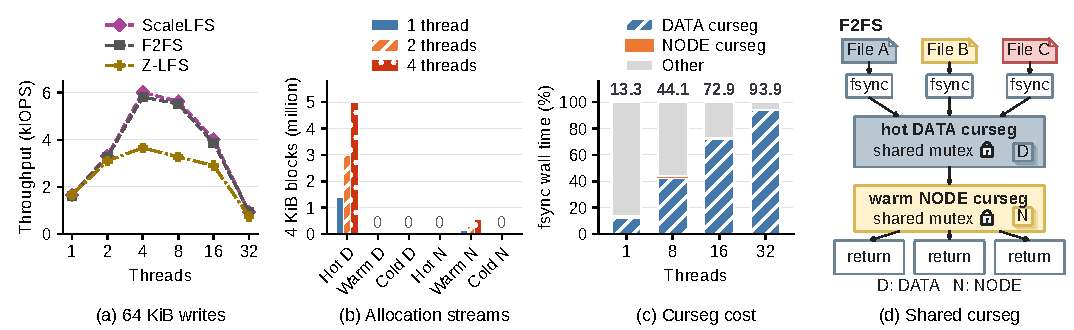
\includegraphics[width=\textwidth]{./figures/compact_motivation64k.pdf}
\caption{Shared allocation with 64\,KiB synchronous updates. (a) Baseline throughput scaling; (b) block counts for six F2FS allocation streams; (c) DATA/NODE curseg intervals within full sampled fsync calls, with combined percentages above bars; (d) schematic of files sharing curseg. D/N denote DATA/NODE in (b). Each numerical panel uses its own measurement protocol.}\label{fig:motivation}
\end{figure*}

Our contributions are:
\begin{enumerate}
\item PACK combines commit closures with parallel appends.
It gathers current writeback and pending mappings, using related NODEs and a terminal to define recoverable updates.
Lanes separate allocation state across updates and support ordered recovery of interleaved commits.
\item Separate append state supports commits and maintenance within finite zone resources.
Leases grant append permission, while a shared physical ledger accounts for active/open occupancy.
Commits return permission before maintenance that may depend on checkpoints or GC; maintenance uses its reserved lane.
\item The implementation increases durable completion rates and reduces extreme tail latency.
On Linux 7.2.9, 4\,KiB synchronous random writes at 32 threads reach 41.27\,kIOPS, 5.58$\times$ F2FS, the fastest baseline under that condition.
With sixteen SQLite databases, transaction throughput reaches 1.94$\times$ the fastest baseline, F2FS, while p99.9 falls 73.4\% below Btrfs, the lowest-latency baseline.
FileMicro synchronous writes and NATS publishes reach about 1.9$\times$ their fastest baselines; extended Varmail also improves mixed file operations.
\end{enumerate}
